\section{Memorable}
\label{sec:method}

A conversation is a sequence of turns $T = (t_1, \dots, t_n)$, each with a speaker, a date and its text $x_i$. Memorable stores $T$ once with fixed code and a local embedder. Its model calls happen at question time (Figure~\ref{fig:method}): a small planner that proposes search queries for the question $q$ and a frozen reader that receives $k$ turns in conversation order and answers. Everything between the two is fixed code, a 33M-parameter embedder and a 278M-parameter cross-encoder, all run on a laptop CPU.

\begin{figure}[t]
\centering
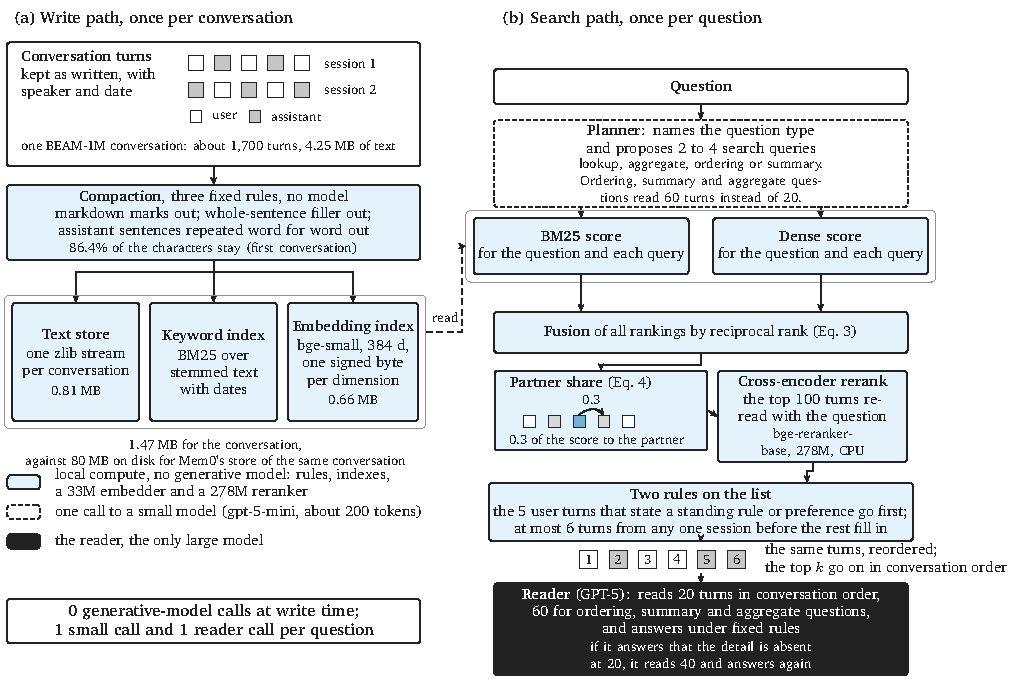
\includegraphics[width=\textwidth]{fig_method.pdf}
\caption{Memorable. (a) The write path runs once per conversation on fixed code and a local embedder. Turns are compacted by three rules, the text is stored with zlib and each turn's embedding as 8-bit integers. (b) The search path runs once per question. A planner proposes two to four queries; keyword and embedding rankings are fused; each turn lends a share of its score to its partner; a cross-encoder rescores the top 100; standing instructions are placed first; at most six turns come from one session; the reader answers from 20 or 60 turns.}
\label{fig:method}
\end{figure}

\subsection{Store}
\label{sec:store}

\paragraph{Compaction.} Assistant prose in a long conversation carries a great deal of markdown decoration, pleasantries and caveats repeated hundreds of times, and each of them costs reader tokens when its turn is retrieved. We remove them with three deterministic maps applied to every turn, $C = R \circ F \circ M$. $M$ strips markdown decoration (heading marks, emphasis stars, horizontal rules, table separator rows and code-fence lines) and replaces table pipes with a spaced bar so that cell contents stay readable. $F$ removes a sentence from either speaker when the whole sentence is a pleasantry or a sign-off, such as ``Certainly!'' or ``Let me know if you need further assistance!''. $R$ removes an assistant sentence longer than 40 characters whose lower-cased, punctuation-stripped form already appeared earlier in the conversation, keeping the first copy. All three maps are string operations. On the first BEAM-1M conversation (1,710 turns, 4.25M characters) the three maps keep 93.1\%, 91.2\% and 86.4\% of the characters in turn, and over all 35 conversations 83\% remain (Figure~\ref{fig:waterfall}). On the 500K development set compaction moved the pass rate by less than two points while cutting the tokens sent to the reader from 23.7K to 19.2K per question.

\paragraph{Storage.} The compacted turns, with their ids, speakers, session indices and dates, are written as one zlib stream per conversation; the session index adds 363 bytes per 1M conversation on average. Each turn's first 256 tokens are embedded once with bge-small-en-v1.5 \citep{xiao2023cpack}, $d = 384$, the vector is unit-normalised, and one signed byte is stored per dimension,
\begin{equation}
\mathbf{q}_i = \mathrm{round}(127\,\mathbf{e}_i), \qquad \hat{s}_i = \mathbf{e}_q^{\top}\mathbf{q}_i / 127 ,
\label{eq:quant}
\end{equation}
so that 384 bytes replace 1,536. The score error is at most $|s_i - \hat{s}_i| \le \|\mathbf{e}_q\|_1 / 254 \le \sqrt{d}/254 \approx 0.077$. We can afford this because the cross-encoder of Section~\ref{sec:search} rescores the top 100 candidates from their text, so the error affects which turns reach that list and leaves their order within it to the cross-encoder; Appendix~\ref{app:int8} compares recall with float and 8-bit vectors. The bytes stored for one conversation are
\begin{equation}
B(T) = |\mathrm{zlib}(C(T))| + n\,d .
\label{eq:bytes}
\end{equation}
Over the 35 BEAM-1M conversations, 159.8~MB of text and 114.6~MB of float vectors become 33.5~MB and 28.7~MB: 62.1~MB stored against 274.4~MB raw, or 1.77~MB per conversation. A stemmed BM25 index over the compacted text \citep{robertson2009bm25}, with each turn's date in its document, is rebuilt from the stored text when a conversation is loaded, so it is left out of $B(T)$.

\subsection{Search}
\label{sec:search}

\paragraph{Planner.} Which turns answer a question depends on its type. A lookup needs the one turn that states a fact, whereas an aggregate, an ordering or a summary needs evidence from many sessions, and a single query rarely reaches them all (Section~\ref{sec:beam}). One call to a small model (gpt-5-mini, about 200 input tokens, about \$0.001 per question) therefore labels the question as a lookup, an aggregate, an ordering (``order'' in the prompt) or a summary and proposes $m \le 4$ search queries $q_1, \dots, q_m$ that together cover it. A question about the days, weeks or months between two events is labelled a lookup, so the reader receives 20 turns; aggregates receive 60.

\paragraph{Fusion.} We rank the turns for the question and for each planner query twice, by BM25 and by embedding cosine, so that a turn can be found by its words or by its meaning. When a turn's date matches a date named in the question, half of the highest BM25 score in that list is added to the turn's BM25 score, which pulls the turns of a named day to the front. Each list is cut to its top 200 and all $2(m+1)$ lists are fused by reciprocal rank \citep{cormack2009rrf},
\begin{equation}
s_i = \sum_{\ell} \frac{1}{60 + r_\ell(i)} ,
\label{eq:rrf}
\end{equation}
where $r_\ell(i)$ is the rank of turn $i$ in list $\ell$. Each turn then lends 0.3 of its score to its neighbour $p(i)$, the other turn of its user-assistant exchange,
\begin{equation}
s'_i = s_i + 0.3\, s_{p(i)} ,
\label{eq:pair}
\end{equation}
because the question often matches one half of the exchange while the answer sits in the other. A local cross-encoder, bge-reranker-base \citep{chen2024bgem3}, reads the question beside the first 1,500 characters of each of the 100 turns with the highest $s'$ and scores how well the turn answers it. The cross-encoder ranking is fused with the earlier ranking by Equation~\ref{eq:rrf} once more, and the 100 candidates stay above every other turn.

\paragraph{Standing rules and a session cap.} Two rules act on the fused list before the reader sees it. The first keeps the user's standing instructions in view. User turns that open with ``always'' or ``never'', or whose first 400 characters contain ``from now on'', ``I prefer'' or ``my preference'', form a pool of standing rules, and the five closest to the question by embedding are placed first, so a rule stated early in the conversation reaches the reader on every later question. The second spreads the read set across sessions: turns are taken from the top of the list, a turn is skipped once six turns from its session have been taken, and the skipped turns fill whatever places remain. The reader receives the first $k = 20$ turns in conversation order, or $k = 60$ for ordering, summary and aggregate questions. If a reader given 20 turns answers that the detail is absent, it is given 40 turns and answers again.

\subsection{Reader}
\label{sec:reader}
The reader (GPT-5) sees each turn, cut to 6,000 characters, with its date and speaker, and answers under fixed rules (Appendix~\ref{app:rules}). The rules about evidence tell it to use only the excerpts, to keep exact names, numbers and dates, to follow standing instructions, and to say that the conversation lacks a detail rather than fill one in. The rules about answers cover the cases a verbatim memory raises that a model-written one has already resolved. The reader prefers the most recent of two conflicting excerpts and says that the fact changed, lists instances with their dates before giving a count, merges repeated mentions of one event, and gives only the most recent value when the question asks for the current one. Four more rules of the same kind, on repeated instructions, relative dates, summaries and the time between two events, are in the full text.

\subsection{Cost}
\label{sec:costmodel}
A memory that a model writes costs $c_w$ per exchange, $N$ in all, and $c_r$ per question, $Q$ in all. Memorable has a write cost of zero and costs $c_p + c_r'$ per question, with $c_p$ the planner call and $c_r'$ the reader:
\begin{equation}
\mathrm{Cost}_{\text{writer}}(Q) = N c_w + Q c_r, \qquad \mathrm{Cost}_{\text{ours}}(Q) = Q\,(c_p + c_r'), \qquad Q^{*} = \frac{N c_w}{c_p + c_r' - c_r} .
\label{eq:cost}
\end{equation}
With the measured values of Section~\ref{sec:cost}, $N c_w = \$7.50$ and $c_p + c_r' = \$0.047$, and an estimated $c_r = \$0.0307$ for Mem0's 200 retrieved facts, the break-even is $Q^{*} \approx 460$ questions per conversation (Figure~\ref{fig:breakeven}). Below it Memorable is cheaper in total; above it Mem0 is, because its reader sees fewer tokens per question. Storage is outside the equation and favours Memorable at every $Q$.
